%%%%%%%%%%%%%%%%%%%% author.tex %%%%%%%%%%%%%%%%%%%%%%%%%%%%%%%%%%%
%
% sample root file for your "contribution" to a proceedings volume
%
% Use this file as a template for your own input.
%
%%%%%%%%%%%%%%%% Springer %%%%%%%%%%%%%%%%%%%%%%%%%%%%%%%%%%


\documentclass{svproc}
\usepackage{marvosym}
%
% RECOMMENDED %%%%%%%%%%%%%%%%%%%%%%%%%%%%%%%%%%%%%%%%%%%%%%%%%%%
%
\usepackage{graphicx}

% to typeset URLs, URIs, and DOIs
\usepackage{url}
\usepackage{hyperref}
\usepackage[english]{babel} 
\usepackage{amsmath} 
\def\UrlFont{\rmfamily}
\providecommand{\doi}[1]{doi:\discretionary{}{}{}#1}

\def\orcidID#1{\unskip$^{[#1]}$}
\def\letter{$^{\textrm{(\Letter)}}$}

\begin{document}
\mainmatter              % start of a contribution
%
\title{On the use of decision trees to identify the local extrema in parallel global optimization algorithms}
%
\titlerunning{Global Optimization ...}  % abbreviated title (for running head)
%                                     also used for the TOC unless
%                                     \toctitle is used
%
\author{K.~A.~Barkalov\inst{1}\letter\orcidID{0000-0001-5273-2471} \and I.~G.~Lebedev\inst{1}\letter\orcidID{0000-0002-8736-0652} \and D.~I.~Silenko\inst{1}\letter\orcidID{0000-0002-2578-9699}}
%
\authorrunning{K.~A.~Barkalov et al.} % abbreviated author list (for running head)
%
%%%% list of authors for the TOC (use if author list has to be modified)
\tocauthor{K.~A.~Barkalov and I.~G.~Lebedev, and D.~I.~Silenko}
%
\institute{Lobachevsky State University of Nizhny Novgorod, Nizhny Novgorod, Russia \\
\email{ \{konstantin.barkalov,ilya.lebedev,silenko\}@itmm.unn.ru}
}

\maketitle              % typeset the title of the contribution

\begin{abstract}
In the present work, the solving of the multidimensional global optimization problems using decision tree to reveal the attractor regions of the local minima is considered. The objective function of the  problem is defined as a ``black box''.  We assume it only to satisfy Lipschitz condition with unknown constant.  Global search algorithm is applied for the search of global minimum in the problems of such type. In the present work, we propose a method for selecting the vicinity of local extrema of the objective  function based on analysis of accumulated search information. Conducting such an analysis using machine learning techniques allows making a decision to run a local  method, which can speed up the convergence of the algorithm.  This suggestion was confirmed by the results of numerical experiments demonstrating the speedup  when solving a series of test problems.
% We would like to encourage you to list your keywords within
% the abstract section using the \keywords{...} command.
\keywords{Global optimization $\cdot$ Multiextremal functions $\cdot$ Parallel computing $\cdot$ Machine learning $\cdot$ Decision tree}
\end{abstract}
%

\section{Introduction}

In the present work, we consider the parallel algorithms for solving the multidimensional global optimization problems. Such problems often arise in the cases, when it is necessary to select the values  of parameters of the mathematical model being investigated, in which the simulation results best fit the experimental data. For solving the problems of this class, many algorithms are known: from the metaheuristic algorithms, based on the  idea of random search \cite{Ferreiro2013,Garcia2014,Langdon2011}, to the deterministic algorithms guarantying convergence to the global minimum \cite{Evtushenko2009,He2008,Paulavicius2011}.  

Since in real global optimization problems each computing of the function value (hereafter called  \textit{a trial}) is a computation-costly operation, one has to reduce the number of such trials. It  can be achieved by intentional choice of variants in the course of search for the optimal solution cutting  off unpromising search subdomains and investigating only these ones, in which the solution of the  problem can be found. The global search algorithm (GSA) is based on this idea. In  the present work, we tried to combine GSA and a local optimization method (Hooke-Jeeves pattern search method) to reduce the number of trials executed. The decision on the run of the local method will be made using a decision tree.

The local optimization algorithms are intended for determining only one of local extrema within a set  of feasible solutions, in which the objective function takes the extremal (maximum or minimum) value.  Among the local methods,  the zero-order methods and the gradient methods (of the 1\textsuperscript{st} order and of the  2\textsuperscript{nd} one) are traditionally distinguished. Note that the application of the first-order methods (not to mention the second one) in the problems  with the ``black-box'' type functions is difficult since the problem of numerical estimating the gradient arises here. Therefore, further we will consider only the zero-order methods. 

In order to determine,  at which moment it is best to run the local method within the framework of the  global search, we will use an algorithm based on a decision tree. At the first search stage, the search information is accumulated in the form of the results of the trials  executed. We used the trial results for training the decision tree that allows obtaining a piecewise constant approximation of the objective function and predicting the objective function behavior on its base.  To do so, we will compare the function values at the points neighboring to the one, which we consider  to be suspicious for a local minimum, and make a decision  whether the next trial point falls into the attractor region of a local minimum or not.

The main part of the paper has the following structure.  In Section \ref{SecPS}, the global optimization problem statement is considered, the basic suggestions  on the objective function are made. In Section \ref{SecA}, the description of the methods and approaches used is given. In particular, in Section \ref{SecGSA},  the main idea of global search algorithm is discussed, its computational rules are given. Section \ref{SecHG} contains the description of the local search method used. The method of constructing the approximation of the function using the decision trees is described in  Section \ref{SecDT}. The novel algorithm combining the global search and the local one on the base of using the decision  trees is presented in Section \ref{SecGSAL}. In the next section,  the features of the asynchronous parallelization scheme of the new algorithm are discussed. Section \ref{SecR} contains the results of experiments, carried out using a parallel computer system  with distributed memory, and a brief conclusion.


\section{Problem statement}\label{SecPS}

Let us consider a problem of searching the global minimum of a function $\varphi(y)$ in a hyperinterval  $D=\{ y\in\ R^N:\ a_i\le\ y_i\le\ b_i,\ 1\le\ i\le\ n \}$. 
\begin{equation} \label{sec:problem}   
	\varphi(y^*) = min\{\varphi(y):y\in D\}, D = \{y \in R^N : a_i \leq y_i \leq b_i, 1 \leq i \leq N \},
\end{equation}
where $a,b \in R$ are given vectors.

Also, assume the function to satisfy the Lipschitz condition with \textit{a priori} unknown constant $L$, that corresponds to limited variation of the function values at limited variation of the argument.   
\begin{displaymath} 
	|\varphi(y_1)-\varphi(y_2)|\leq L\parallel y_1-y_2 \parallel ,y_1,y_2 \in D, 0<L< \infty. 
\end{displaymath}
This suggestion can be interpreted (with respect to the applied problems ) as the reflection of limited  power generating the changes in the system being simulated.

The numerical solving of the problem (\ref{sec:problem})  is reduced to constructing an estimate  $ y_k^\ast\in D$ matching some concept of nearness to the point $y^\ast$ (for example,  ${||y^\ast-y}_k^\ast||\le\ \varepsilon$, where $\varepsilon\geq0$ is a predefined accuracy) based on a  finite number $k$ of the objective function values computed. With respect to the class of the considered problems, it is suggested that the objective function $\varphi(y)$ can be defined algorithmically, as a result of executing some subroutine or library.

The solving of the multiextremal optimization problems is much more computation-costly  as compared  to other types of optimization problems since the global optimum is an integral characteristic of the  problem being solved and requires investigating the whole search domain. As a result, the search of the  global optimum is reduced to constructing some coverage (grid) in the search domain and the choice of  the best function value on this grid. When using the uniform grids, the computation costs of solving the  problem grow exponentially with increasing dimensionality.



\section{The algorithms used}\label{SecA}

The main idea of the approach to constructing more efficient nonuniform grid is that its points are  computed sequentially while the objective function is considered as a realization of some random process. The decision rules of the grid building algorithm are constructed in such a way that the next  grid point corresponds to the global minimum point of the mathematical expectation of the function  values. This point is stored in the list of known values, and the iterations are repeated until the stop criteria is satisfied: either the distance between the trial points becomes less than a  predefined value or a preset maximum number of iterations is achieved \cite{fio_bib10}.

When solving the multidimensional problems, the dimensionality reduction (i.e. the reduction of the  multidimensional problem to an equivalent one-dimensional one) using Peano curves is applied. These  ones allow reducing a multidimensional optimization problem in the domain $D$  to a one-dimensional  minimization problem within the interval $[0, 1]$
\begin{displaymath}
	\varphi(y(x^\ast))\ =\min\{\varphi(y(x)): x\in [0,1]\},
\end{displaymath}
where the function $\varphi(y(x^\ast))$ satisfies more general H{\"o}lder condition
\begin{displaymath}
	\left|\varphi (y \left(x_1\right))- \varphi (y \left(x_2\right)\right )|\le\ H\left|x_1-x_2\right|^\frac{1}{N},\ x_1,\ x_2\epsilon[0,1].
\end{displaymath} 


Therefore, instead of the initial problem of minimizing the function $\varphi(y)$ in the domain $D$,  we can consider the minimization of the one-dimensional function $f(x)=\varphi(y(x))$ satisfying  the H{\"o}lder condition for $ x\in [0,1]$.



\subsection{Multidimensional parallel global search algorithm}\label{SecGSA}

The main steps of the parallel global search algorithm are as follows.

At the preliminary step, $p$ trials are executed in parallel in arbitrary internal points $x^1, ...,x^p$ of  the interval $[0,1]$ that corresponds to the first iteration of the algorithm. 

If $n \geq 1$ iterations are completed, which correspond to $k=k(n)$ trials executed at the points $x^i, 1\leq i\leq  k$, then the points $x^{k+1},\ldots,x^{k+p}$ of the search trials at the next $(n+1)^{\rm  th}$ iteration will be computed as the result of performing the following operations.

\begin{enumerate}
	
	\item  Renumber (by the lower indices) the points $x^i, 1\leq i\leq k$ as well as the boundary points of  the interval [0,1] in increasing order of the coordinate  
	\begin{equation} 
		\label{agp1_sort} 	0=x_0<\ x_1<\ ...\ <x_{k+1}=1. 	
	\end{equation} 
	and juxtapose them with the values $z_i=f(x_i)$. 
	
	\item  Compute current lower estimate $M$ of the unknown H{\"o}lder constant $H$:  
	\begin{equation} 
		\label{agp2_mu} 	\mu=max\left\{\frac{|z_i-z_{i-1}|}{{{(x}_i-x_{i-1})}^{1/N}},\ i=1,\ldots,k\right\},\ M=\  \left\{\begin{matrix}r\mu,\ \mu>0,\\1,\ \mu=0,\\\end{matrix}\right.\ 	
	\end{equation} 
	where $r>1$ is a parameter of algorithm. This parameter controls the reliability of the algorithm: the  higher values of $r$ ensure guaranteed finding of the global minimum, the choice of lower value speeds up the convergence of the algorithm. 
	
	\item  For each interval $(x_{i-1},x_i), 1\leq i\leq k+1,$ compute the value $R(i)$ called \textit{a  characteristic} of the interval according to the formulae 
	\begin{equation} 
		\label{agp3_R1} R(1)=2\Delta_1-4\dfrac{z_1}{M}, \; R(k+1)=2\Delta_{k+1}-4\dfrac{z_k}{M}, 
	\end{equation} 
	\begin{equation} 
		\label{agp3_Ri} R(i)=\Delta_i+\dfrac{(z_i-z_{i-1})^2}{M^2\Delta_i}-2\dfrac{z_i+z_{i-1}}{M},1<i<k+1, 
	\end{equation} 
	where \(\Delta_i=(x_i-x_{i-1})^\frac{1}{N}\).
	
	\item   Arrange the characteristics $R\left(i\right),\ 1\leq i \leq k+1,$ in the non-increasing order 
	\begin{equation} 
		\label{agp4_R_sort} 	R\left(t_1\right)\geq\ R\left(t_2\right)\geq...\geq\ R\left(t_k\right)\geq\ R(t_{k+1}),\  
	\end{equation} 	
	and select $p$ intervals with the indices $t_j,\ 1\le\ j\le\ p$ with the largest values of characteristics.
	
	\item Compute the points $x^{k+j},\ 1\leq j\leq p$ in the selected intervals according to the formulae
\begin{equation}
	\label{agp5_x1}
	x^{k+j}=\frac{x_{t_j}+x_{t_j-1}}{2},\ t_j=1,\ t_j=k+1,
\end{equation}	
\begin{equation}
	\label{agp4_xi}	
	x^{k+1}=\frac{x_{t_j}+x_{t_j-1}}{2}-sign\left(z_{t_j}-z_{t_j-1}\right)\frac{1}{2r}\left[\frac{\left|z_{t_j}-z_{t_j-1}\right|}{\mu}\right]^N,\ 1<t_j<k+1.
\end{equation}
	
\end{enumerate}

The next $p$ trials are executed in parallel at the points $x^{k+j},\ 1\leq j\leq p$, computed according  to the formulae (\ref{agp5_x1}), (\ref{agp4_xi}). Upon completing the trials, the results of these ones  are stored in the information database, and the algorithm goes to computing new trial points.
Note that as a rule the process of executing a trial in the applied optimization problems is much more  computation-costly as compared to computing the trial point.

The algorithm stops in the case if the condition \(\Delta_{t_j} < \varepsilon\) is satisfied for even a  single value $t_j,\ 1\le\ j\le\ p$ from (\ref{agp4_R_sort}). This stop criterion (along with the criterion limiting the number of executed iterations usual for the  iteration methods) is used in the applied optimization problems, in which the global minimum point $x^*$ is unknown a priori. 

When solving the test problems, in which the global minimum point $y^*$ is known, we can use the stop criterion upon falling into the vicinity of the global minimum as well. In this case, the method  stops if the condition $\left\|y(x_{t_j})-\ y^\ast\right\| < \varepsilon$ is satisfied even for one value of $t_j,\  1\le\ j\le\ p$, from (\ref{agp4_R_sort}). 

As the final estimate of the global optimizer of the considered problem, the values 
\begin{equation} 
	f_k^*=\min_{1\leq i \leq k}f(x_i), \; x_k^*=arg \min_{1\leq i \leq k}f(x_i). 
\end{equation} 
are taken. 

The substantiation of this method of organization of computations see in \cite{Strongin2013}. The  modifications taking into account the presence of inequality constraints as well as the information on the derivative of the objective function are presented in \cite{Barkalov2002,Gergel1997}.



\subsection{Hooke--Jeeves method}\label{SecHG}

The Hooke--Jeeves pattern search algorithm belongs to the class of zero-order methods. Its computation rules are a  combination of the investigating search (to select the direction) and search in the direction selected  \cite{NelderMead,Himmelblau75}.

The investigating search is performed as follows. 
\begin{enumerate} 
\item	The step value is determined (it is different for each coordinate and can be varied in the course  of search).  
\item	The search step is considered to be successful if the value of the objective function at the check  point doesn't exceed the value of the objective function at the initial point.  
\item	Otherwise, it is necessary to return to the previous item and make a step in the reverse direction.  
\item	After making the steps in all $N$ coordinates, the investigating search is completed. The point  obtained is called the base point. 
\end{enumerate}

With regard to the search in a direction, it consists in performing a step from the base point found  during the investigating search along the straight line direction connecting this one with the previous  base point. The magnitude of this step is defined by a parameter set in advance.

\begin{figure}[!h] 
	\begin{center} 
		\begin{minipage}[h]{0.8\linewidth} 
			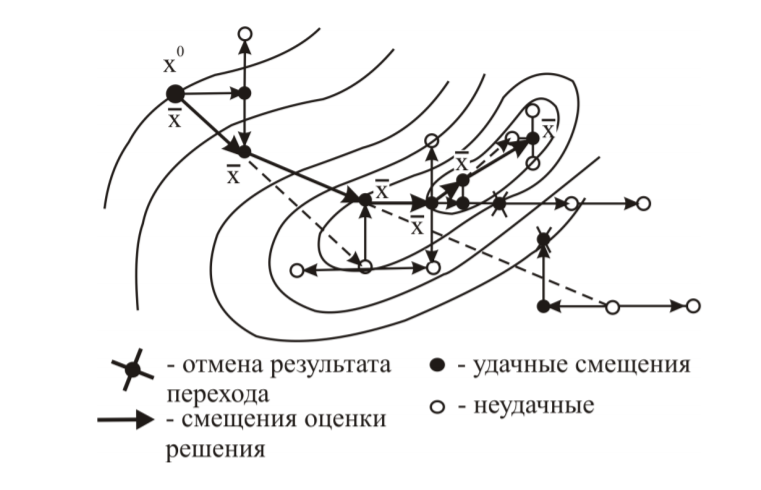
\includegraphics[width=1\linewidth]{figure/fig1.png} 
			\caption{An example of iterations of the Hooke-Jeeves algorithm} %%  подпись к рисунку 
			\label{fig:fig1} 
		\end{minipage} 
	\end{center} 
\end{figure}	



\subsection{Decision tree}\label{SecDT}

The decision tree is a tool used for an automated analysis of big data arrays, which is applied in the  machine learning. Decision tree is a binary tree (a tree, in which each non-leaf node has two child nodes). It can be used for solving the classification problems as well as the regression ones. When solving  the classification problems, each leaf of the tree is marked by a class label, and several leafs can have  the same labels. In the case of constructing a regression, a constant is assigned to each leaf of the tree.   Therefore, the approximating function obtained is a piecewise-constant one. In our case, the decision tree constructs the function $\psi(y)$ as a piecewise-constant  approximation of $\varphi(y)$ in the search domain. Let us denote the value  computed by the  decision tree at the point $y$ as $z' = \psi(y)$.

When implementing the algorithm for finding the attraction areas of the local  minima, we used the algorithms from OpenCV library to construct decision tree. OpenCV is an open source library of the algorithms of computer vision, image processing, and  general-purpose numerical algorithms. More details on the decision tree can be found  in \cite{Opencv}.

\section{Combination of local and global search algorithms for solving multidimensional  problems}\label{SecGSAL}

In the current section, let us present a detailed description how we used the decision tree for finding  the attraction areas of the local extrema.  In the course of running GSA, it is necessary to determine whether it is worth to use current point as a  start one for the local method or not. To do so, one can check the points of adjacent trials. If among  these ones there are no points at which the function values are lower than in current one, one  can suggest that we are in the attractor of a local minimum. In this case, we can run the local method  from current point, which will rapidly converge to a local minimum of the function.  We can do it in the multidimensional space only, not in one-dimensional interval after the  dimensionality reduction.  First, the reduced function $\varphi(y(x))$ changes its properties: one local minimum in the  multidimensional space may divide into a set of minima after the dimensionality reduction.  Second, after the use of the mapping $y(x)$, we can lose the information on the mutual arrangement of  the points in the original space. The points located close to each other in the multidimensional space  may appear to be essentially separated in the one-dimensional interval.




Therefore, we will determine the attraction areas of the local extrema in the original multidimensional space. However, the determining of the adjacent points in the multidimensional space is quite expensive in terms of computing resources. To do so, we will use the decision tree. 

After completing a certain number of trials (for example, $100\ \ast\ N$), let us use all accumulated  points to initialize a suitable data structure and training the decision tree on its base. To make the  determining the adjacent points easier, we construct a uniform grid with certain step in each coordinate.  Next, we compute the values of the approximation of the objective function in these points  using the decision tree. Now, having a uniform grid of points and knowing the function values in each  point, let us find the closest point to the initial one (from the viewpoint of the Euclidian distance). This  closest point is a projection of the initial point onto the uniform grid, on which its neighbors can be  determined easily. Since the decision tree constructs the approximation of the initial function (even  piecewise constant), we can estimate the function values in the areas, in which the trials haven't been  executed earlier.

When considering the neighbors, it is necessary to take into account the following. If even a single  neighbor has a lower function value than current point, there is no need to run the local method. If at  even a single neighboring point the function value is the same as at the current one, this point must be also checked (i.e. to find all its neighbors and to check these ones in the same way). Only in the case when  all function values at the neighboring points are greater than at the current point, we can run the local  method.

%Fig. \ref{fig:fig2} presents a contour plot of an objective function and the trial points; Fig.  \ref{fig:fig2_2} presents corresponding decision tree. 



\section{Asynchronous algorithm parallelization scheme}\label{SecASP}

The method of parallel computing described in  previous section implies synchronous  performing of $p$ search trials at the points computed at current iteration. The next iteration will be  started only upon completing all trials. In the case of different computation costs of executing the trials at different points of the search  domain, this approach may lead to a disbalance of the computing jobs.  This drawback can be corrected by introduction of asynchrony. The idea of the asynchronous scheme is not to wait for completing all $p$ trials but to initiate the  execution of a new trial immediately upon completing one of the trials. 

Let us assume that the master process computes one point of the next trial at every iteration and sends  it to the worker process to execute the trial. Note that executing a trial by the worker process in  the applied optimization problems is much more computation costly than the choice of a new trial point  by the master process. Therefore, the idle time of the processes will be negligible. In this  case (unlike the synchronous parallel algorithms) total number of trials executed by each worker  process will depend on the computation costs for executing particular trials and cannot be estimated in  advance. When describing the parallel algorithm, let us assume that we have $p+1$ computational  processes at our disposal: one master and $p$ workers.

In the beginning of search, the master process (assume it to have the identifier $0$) initiates parallel  execution of $p$ trials in $p$ different points of the search domain.
Two of these points are the boundary ones, the rest are the internal points, i.e. at the points  $\{y\left(x^1\right),y\left(x^2\right),\ldots,y\left(x^p\right)\}$ where $x^1=0,x^p=1,x^i\in\left(0,1\right),i=2,\ldots,p-1$.

Now assume $k\geq0$ trials to be completed, and the worker processes are performing the trials at the points $y\left(x^{k+1}\right),\;y\left(x^{k+2}\right),\ldots,\;y\left(x^{k+p}\right)$.

Each worker process having completed the computing of the function at some time moment sends  the computed value to the master process. In turn, the master process selects a new point  $x^{k+p+1}$ for the worker process according to the rules described below. Note that in this case  we will have a set of preimages of the trial points  $I_k=\left\{x^{k+1},x^{k+2},\ldots,x^{k+p}\right\}$, in which the trials have been already started but haven't been completed yet.

So far, the parallel asynchronous global optimization algorithm using decision tree to find the local  extrema attractors consists of the following steps.

\begin{enumerate} \item Arrange in the increasing order (by the lower indices) the set of preimages of the trial points
	\begin{displaymath} 
		X_k=\left\{x^1,x^2,\ldots,x^{k+p}\right\}, 
	\end{displaymath} 
	containing all points, in which the trials either have been completed or are being executed, i.e. get an  ordered set 
	\begin{displaymath} 
		0=x_1<x_2<\ldots<x_{k+p}=1. 
	\end{displaymath} 
	
	\item Compute the values 
	\begin{displaymath} 
		M_1=\max{\left\{\frac{\left|z_i-z_{i-1}\right|}{\left(x_i-x_{i-1}\right)^{1/N}}:x_{i-1}\notin  I_k,x_i\notin I_k,2\le i\le k+p\right\}}, 
	\end{displaymath} 
	\begin{displaymath} 
		M_2=\max{\left\{\frac{\left|z_{i+1}-z_{i-1}\right|}{\left(x_{i+1}-x_{i-1}\right)^{1/N}}:x_i\in  I_k,2\le i<k+p\right\}}, 
	\end{displaymath} 
	\begin{displaymath} 
		M=\max{\{}M_1,M_2\}, 
	\end{displaymath} 
	where $ z_i=\varphi\left(y\left(x_i\right)\right)$ if $x_i\notin I_k,\;1\le i\le k+p$. The values $z_i$ at the points $x_i\in I_k$ are undefined since the trials at the points $x_i\in I_k$ haven't been completed yet. If the value of $M$ equals to $0$, set $M=1$.
	
	\item Juxtapose each interval $\left(x_{i-1},x_i\right),\;x_{i-1}\notin I_k,x_i\notin I_k,\;2\le i\le  k+p$, with its characteristic $R\left(i\right)$ computed according to the formula 
	\begin{displaymath} 
		R\left(i\right)=rM\Delta_i+\frac{\left(z_i-z_{i-1}\right)^2}{rM\Delta_i}-2\left(z_i+z_{i-1}\right), 
	\end{displaymath} 
	where $\Delta_i=\left(x_i-x_{i-1}\right)^{1/N}$ and $ r>1$ is the reliability parameter of the method.
	
	\item Select the interval $\left[x_{t-1},x_t\right]$, which corresponds to the highest characteristic, i.e.
	\begin{displaymath} 
		R\left(t\right)=\max{\left\{R\left(i\right):\;x_{i-1}\notin I_k,x_i\notin I_k,\;2\le i\le k+p\right\}}. 
	\end{displaymath} 
	
	
	\item Define a new trial point $y^{k+p+1}=y\left(x^{k+p+1}\right)$, the preimage of which is  $x^{k+p+1}\in\left(x_{t-1},x_t\right)$, according to the formula 
\begin{displaymath}
	x^{k+p+1}=\frac{x_t+x_{t-1}}{2}-\mathrm{sign}\left(z_t-z_{t-1}\right)\frac{1}{2r}\left[\frac{\left|z_t-z_{t-1}\right|}{M}\right]^N.
\end{displaymath}
	
	
	\item Get the computed function value from the process $j$, add new trial $z_j = f(y(x_j))$ to the set  $V$. 
	
	%X_k=\left\{x^1,x^2,\ldots,x^{k+p}\right\}
	
	\item If $k\ <\ 100 N$, return to Step 1.
	
	%\item  If the decision tree is used not in the first time, go to Step 15.
	
	\item Create the decision tree using the set $I_k$, get the approximating function $\psi(y)$.
	
	\item If the decision tree is used for the first time, construct a uniform grid 
	
	\begin{displaymath} 
		Y'=\{ y'\in\ R^N:\ a_i\le\  {y'_i}^k \le\ b_i,\ 1\le\ i\le\ N,\ 1\le k\le\ \sqrt[N]{300}  \} 
	\end{displaymath} 
	
	
	\item Compute the approximation values: $Z' = \{ z'=  \psi(y'), y' \in Y'\}$
	
	\item For all points $y'\in V$:
	
	Find the points $y'_q$ closest to $y'$,
	
	Make a detour of the neighbors $y'_q$ according to the principle described above.
	
	If no one neighbor point has a lower value than in $y'_q$, run the local method.
	
	Clear the set $V$.
	
\end{enumerate}

Upon computing the next trial point, the master process adds it to the set $I_k$ and sends to the  worker process, which initiates the new trial in this point. The master process stops the algorithm, if one of the two conditions is satisfied: $\Delta_t<$ or  $k+p>K_{max}$. The real value $\epsilon>0$ and the integer value $K_{max}>0$ are the parameters of the algorithm  and correspond to the accuracy of the search and the maximum number of trials, respectively.

\begin{figure}[ht!]
	
	\begin{center} 
				\begin{minipage}[h]{0.9\linewidth} 			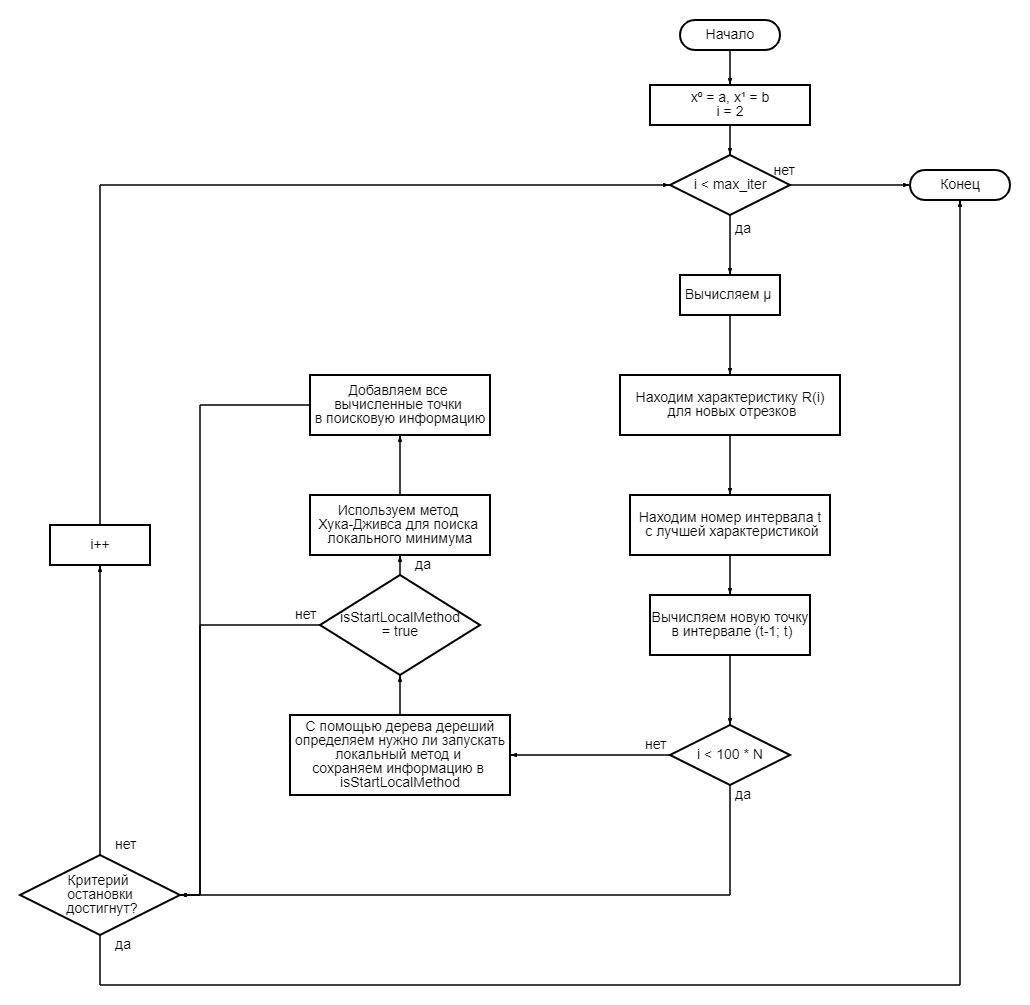
\includegraphics[width=1\linewidth]{figure/fig3.png}
					 			\caption{Block scheme of combined GSA and Hooke-Jeeves method using the  decision tree} %% подпись к рисунку 			\label{fig:fig3}
				 \end{minipage}
	\end{center}
\end{figure}





% переводить до этого раздела
\section{Numerical Experiments}\label{SecR}


The numerical experiments were carried out on Lobachevsky supercomputer. Each supercomputer  node had two processors Intel Sandy Bridge E5-2660 2.2 GHz, 64 Gb RAM. 

In the experiments, we used GKLS generator of test problems, which can generate multiextremal  optimization problems with known properties: the global minimum point, the number of local minima,  etc.

To demonstrate the efficiency of  investigated global search algorithm, here we present the results of  comparing this one with well known methods DIRECT and DIRECTl. Table \ref{tab:1} presents the averaged numbers of iterations executed by respective methods when  solving a series of GKLS problems. The sign «>» points to the situation when not all problems are  solved. In these cases, the numbers of non-solved problems are given in brackets. As one can see,  GSA overcomes DIRECT and DIRECTl methods in average number of iterations necessary for  solving the problems with the same precision.

\begin{table}[!ht]
    \caption{Averaged number of iterations}
    \label{tab:1}
    \centering
    \begin{tabular}{|l|l|l|l|l|}
    \hline
        N & Problem class & DIRECT & DIRECTl & GSA  \\ \hline
        4 & Simple & >47282 (4) & 18983 & 11953  \\ \hline
        ~ & Hard & >95708 (7) & 68754 & 25263  \\ \hline
        5 & Simple & >16057 (1) & 16758 & 15920  \\ \hline
        ~ & Hard & >217215 (16) & >269064 (4) & >148342 (4)  \\ \hline
    \end{tabular}
\end{table}


%Ниже приведены результаты сравнения двух параллельных алгоритмов --- асинхронного GSA и его модификации с использованием decision tree и локального метода Хука-Дживса. Численное сравнение проводилось на классах функций Simple и Hard размерности 2, 3, 4 и 5 из \cite{Sergeyev2006}. Критерием остановки служило попадание точки очередного испытания trial в $\varepsilon$ окрестность истинного глобального минимума. 
%В таблице \ref{tab:2} представлено среднее количество итераций и ускорение по времени относительно последовательного запуска. Распараллеливание  осуществлялось с применением  MPI. При этом запуск производился на 4 процессах, а следовательно, на каждой итерации вычислялось 3 точки. Значение в скобках (если оно есть) показывает количество не решенных задач. Это означает, что было достигнут максимум по числу проводимых итераций, но в окрестность глобального минимума точка так и не попала.


Below, the results of comparing two parallel algorithms --- asynchronous global search algorithm  (GSA) and its modification using the decision tree to find the attractor areas of the local minima  (Decision Tree) are presented. The numerical comparison was performed on two classes of the GKLS  functions (Simple and Hard) of dimensionalities 2, 3, 4, and 5 from \cite{Sergeyev2006}. The stop  criterion for the algorithms was the falling of the next trial points into the $\varepsilon$-nearness of  true global minimum.  In Table \ref{tab:2}, the averaged numbers of iterations executed by the algorithms when solving the  problems and the values of speedup in time relative to the sequential run are compared. The  parallelization was performed using MPI technology, the run was performed on 8 processes.




\begin{table}[h!]
	\caption{Averaged numbers of iterations and averaged numbers of trials executed by different 
		algorithms}
	\label{tab:2}
	\centering
	\begin{tabular}{|c|c|c|c|c|c|}
		\hline
		
		N & Problem class & \multicolumn{2}{c|}{Averaged number of iterations} & \multicolumn{2}{c|}{Speedup} \\ \hline
		& ~ & GSAA & Decision tree & GSAA & Decision tree \\ \hline
		& Simple & 3823,1   & 485,6  & 7,4   & 12,7 \\ \hline
		2  & Hard & 787,6    & 304,2  & 13,8  & 14,9 \\ \hline
		& Simple & 5700,5   & 720,1  & 5,6   & 14,2  \\ \hline
		3  & Hard & 2411,9   & 634,3  & 5,0   & 5,9  \\ \hline
		& Simple & 31101,5  & 1037,4 & 5,1   & 7,1  \\ \hline
		4  & Hard & 10418,1  & 816,2  & 6,9   & 5,0  \\ \hline
		& Simple & 163313,5 & 1204,2 & 4,8   & 4,1 \\ \hline
		5  & Hard & 27524,5  & 999,4  & 4,6   & 6,3  \\ \hline
	\end{tabular}
\end{table}


As one can see from Table \ref{tab:2},  the iteration speedup is large enough for the problems of any  dimensionality. 

So far, as a result of the work done, we succeeded to combine the global search algorithm with a local  optimization method.  Unlike the known multistart schemes, the decision to run the local method is made using the decision  tree. The use of such a combination of methods allows accelerating the work of algorithm considerably. 

The parallel version of the algorithm preserves the properties of its sequential prototype that was  confirmed by he numerical experiments on solving a series of several hundred problems of various  dimensionalities. The scheme we proposed allows utilizing the advantages of both approaches – of the  parallelization as well as of fast search of local extrema.

%
% ---- Bibliography ----
%
\bibliographystyle{spmpsci}
\bibliography{bibliography}{}


\end{document}
